\documentclass{article}
\usepackage{tikz, comment}
\usepackage{pifont}
\usepackage{fontspec}
\usetikzlibrary{arrows, decorations.markings, decorations.pathreplacing}
\begin{comment}
:Title: Not defined yet
:Tags: cardioid;focus of a parabola;tangent line;slope of a curve;segment of a circle
:Prob: 0.5222;0.4821;0.4722;0.472;0.4613
:Author: Prof.Hu Ji-shan, HKUST
:Slug: No name yet

Description Here.........
\end{comment}
\begin{document}\centering

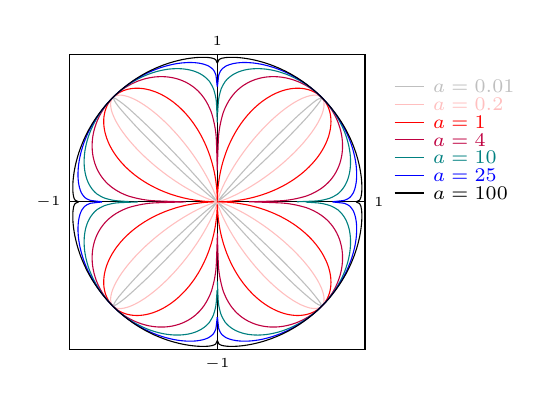
\begin{tikzpicture}[>=latex,xscale=0.375*10/2, yscale=0.375*10/2][font=\sf\small]

%\draw[xstep=1cm,ystep=1cm,color=gray!20] (-2, -2) grid (2, 2);

\draw[] (-1, 0) -- (1, 0);
\draw[] (0, -1) -- (0, 1);

\node[left] at (-1, 0) {\tiny$-1$};
\node[right] at (1, 0) {\tiny$1$};
\node[below] at (0, -1) {\tiny$-1$};
\node[above] at (0, 1) {\tiny$1$};

\draw [lightgray] (1.2, {0.9-1*0.12}) --++(0.2, 0)node[right] {\scriptsize$a=0.01$};
\draw [pink] (1.2, {0.9-2*0.12}) --++(0.2, 0)node[right] {\scriptsize$a=0.2$};
\draw [red] (1.2, {0.9-3*0.12}) --++(0.2, 0)node[right] {\scriptsize$a=1$};
\draw [purple] (1.2, {0.9-4*0.12}) --++(0.2, 0)node[right] {\scriptsize$a=4$};
\draw [teal] (1.2, {0.9-5*0.12}) --++(0.2, 0)node[right] {\scriptsize$a=10$};
\draw [blue] (1.2, {0.9-6*0.12}) --++(0.2, 0)node[right] {\scriptsize$a=25$};
\draw [black] (1.2, {0.9-7*0.12}) --++(0.2, 0)node[right] {\scriptsize$a=100$};

\clip[draw] (-1, -1) rectangle (1, 1);

\draw[lightgray, samples=300, smooth, domain=0:2*pi, variable=\t] %a=0.01
plot ({(abs(sin(2*\t r)))^(1/0.01)*cos(\t r)}, {(abs(sin(2*\t r)))^(1/0.01)*sin(\t r)});

\draw[pink, samples=200, smooth, domain=0:2*pi, variable=\t] %a=0.2
plot ({(abs(sin(2*\t r)))^(1/0.2)*cos(\t r)}, {(abs(sin(2*\t r)))^(1/0.2)*sin(\t r)});


\draw[red, samples=200, smooth, domain=0:2*pi, variable=\t] %a=1
plot ({(abs(sin(2*\t r)))^(1/1)*cos(\t r)}, {(abs(sin(2*\t r)))^(1/1)*sin(\t r)});

\foreach \n in {1,2,3,4}
{
\begin{scope}[rotate around={(\n)*90:({0}, {0})}]
\draw[purple, samples=100, smooth, domain=0.001:pi/2-0.001, variable=\t] %a=4
plot ({1/((abs(sin(2*\t r)))^(-1/4))*cos(\t r)}, {1/((abs(sin(2*\t r)))^(-1/4))*sin(\t r)});
\end{scope}
};

\foreach \n in {1,2,3,4}
{
\begin{scope}[rotate around={(\n)*90:({0}, {0})}]
\draw[teal, samples=200, smooth, domain=0.001:pi/2-0.001, variable=\t] %a=10
plot ({1/((abs(sin(2*\t r)))^(-1/10))*cos(\t r)}, {1/((abs(sin(2*\t r)))^(-1/10))*sin(\t r)});
\end{scope}
};

\foreach \n in {1,2,3,4}
{
\begin{scope}[rotate around={(\n)*90:({0}, {0})}]
\draw[blue, samples=150, smooth, domain=0.001:pi/2-0.001, variable=\t] %a=25
plot ({1/((abs(sin(2*\t r)))^(-1/25))*cos(\t r)}, {1/((abs(sin(2*\t r)))^(-1/25))*sin(\t r)});
\end{scope}
};

\foreach \n in {1,2,3,4}
{
\begin{scope}[rotate around={(\n)*90:({0}, {0})}]
\draw[black, samples=150, smooth, domain=0.001:pi/2-0.001, variable=\t] %a=100
plot ({1/((abs(sin(2*\t r)))^(-1/100))*cos(\t r)}, {1/((abs(sin(2*\t r)))^(-1/100))*sin(\t r)});
\end{scope}
};

\end{tikzpicture}
\end{document}